\section{Case Study}

\begin{frame}[fragile,allowframebreaks]{Open Source Projects}
    
\begin{figure}
    \centering
    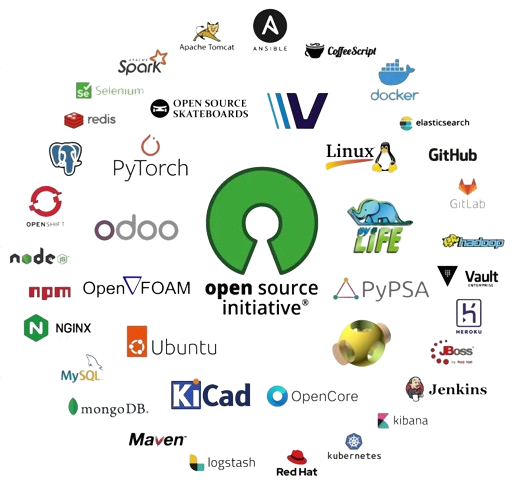
\includegraphics[width=0.42\linewidth]{assets/signal-2024-03-12-131914_002.png}
    % \caption{Open Source Projects}
    % \label{fig:enter-label}
\end{figure}

\end{frame}

\begin{frame}[fragile,allowframebreaks]{Enterprise Resource Planning Systems}
    
\begin{figure}
    \centering
    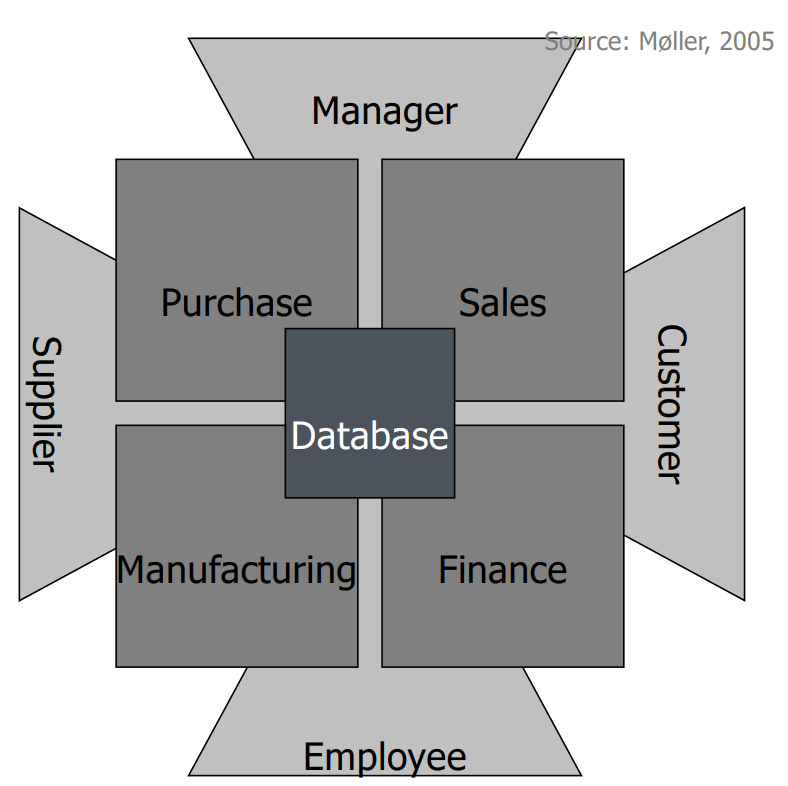
\includegraphics[width=0.40\linewidth]{assets/ERP.png}
    % \caption{Open Source Projects}
    % \label{fig:enter-label}
\end{figure}

\end{frame}

\begin{frame}[fragile,allowframebreaks]{SAP}
    
\begin{figure}
    \centering
    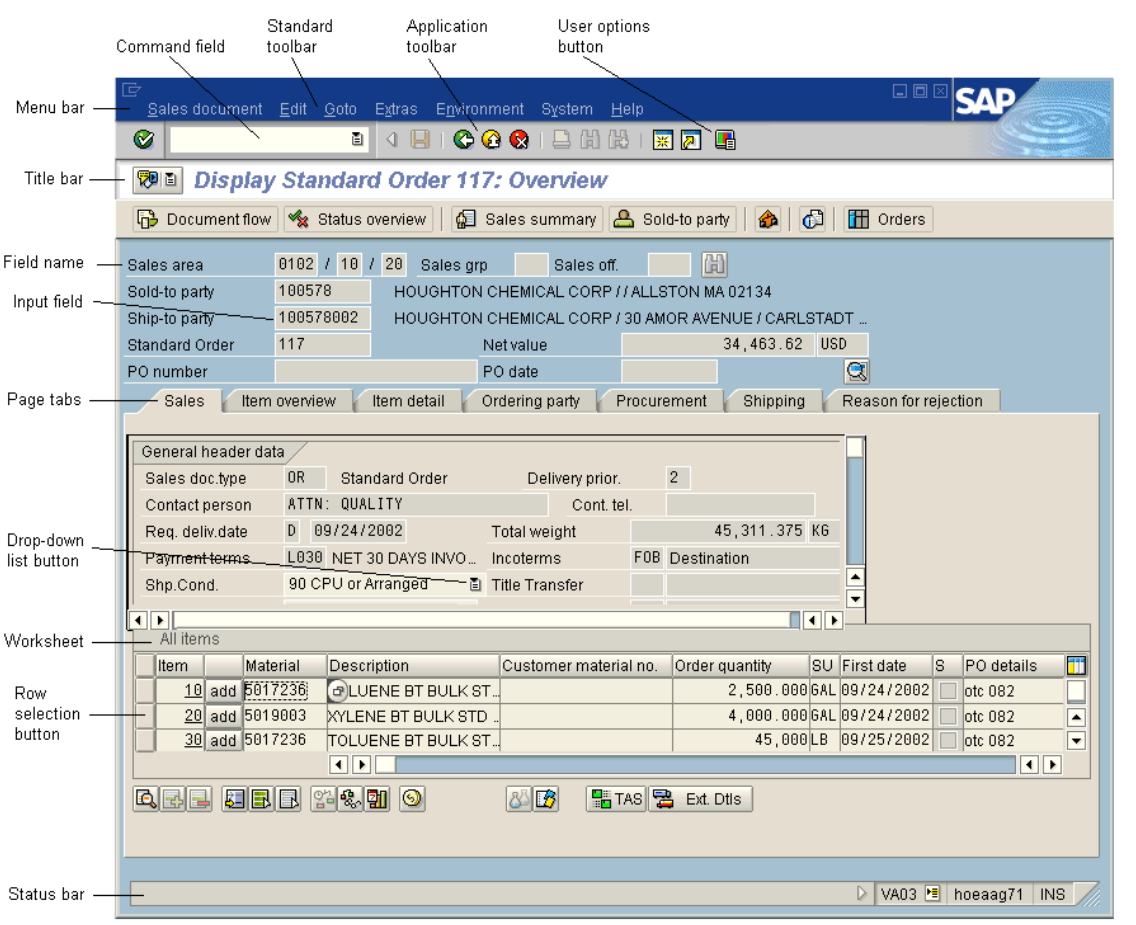
\includegraphics[width=0.50\linewidth]{assets/SAP.png}
    % \caption{Open Source Projects}
    % \label{fig:enter-label}
\end{figure}

\end{frame}
\begin{frame}[fragile,allowframebreaks]{Odoo}
    
\begin{figure}
    \centering
    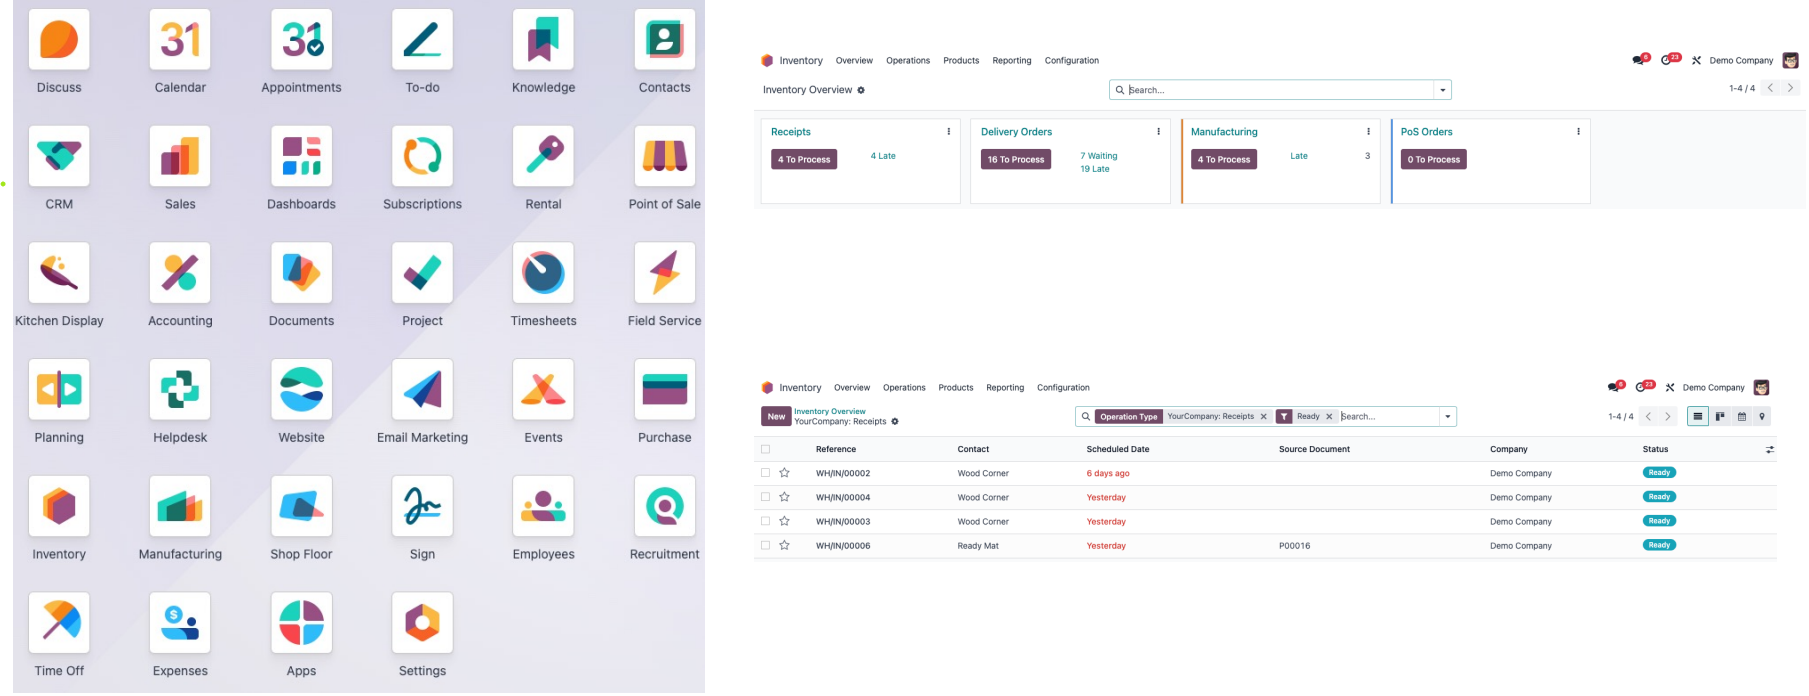
\includegraphics[width=0.90\linewidth]{assets/OdooInterface.png}
    % \caption{Open Source Projects}
    % \label{fig:enter-label}
\end{figure}

\end{frame}

\begin{frame}[fragile,allowframebreaks]{Odoo Key Characteristics}
\begin{itemize}
    \item Transparency
    \item Collaboration
    \item Community-driven Development
    \item Transparency
    \item Freedom to Use and Modify
    \item Licensing
\end{itemize}
    
\end{frame}

\begin{frame}[fragile,allowframebreaks]{Price Comparison}
    
\begin{figure}
    \centering
    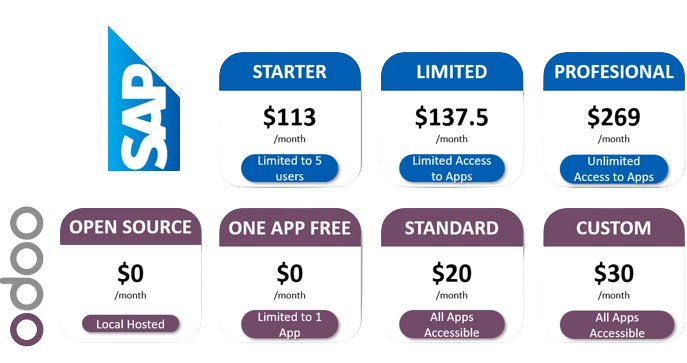
\includegraphics[width=0.70\linewidth]{assets/OdooPrices-removebg-preview.png}
    % \caption{Open Source Projects}
    % \label{fig:enter-label}
\end{figure}
\end{frame}

\begin{frame}[fragile,allowframebreaks]{What is TensorFlow?}
    \begin{columns}[T]
        \column{0.99\textwidth}
            \vspace{1cm}
            \begin{itemize}
                \item Platform for machine learning
                \begin{itemize}
                    \item Machine learning library
                \end{itemize}
                \item Free and open source
                \begin{itemize}
                    \item License: Apache license 2.0
                    \item Initially from Google
                \end{itemize}
            \end{itemize}
        
         \column{0.01\textwidth}
             \vspace{-1cm}
             \hspace*{-4cm}
             
\includegraphics[width=4cm]{assets/TensorFlow_logo_tp.png}
    \end{columns}
\end{frame}

\begin{frame}[fragile,allowframebreaks]{What is TensorFlow?}
    \begin{columns}[T]
        \column{0.99\textwidth}
            \vspace{1cm}
                \begin{itemize}
                    \item Data flow graphs
                    \begin{itemize}
                        \item ML algorithms as a graph of connected operations
                        \item Quick and intuitive work flow
                    \end{itemize}
                \item Works with Python, C++ etc.
                \end{itemize}
         \column{0.01\textwidth}
            \vspace{.5cm}
            \hspace*{-4cm}
            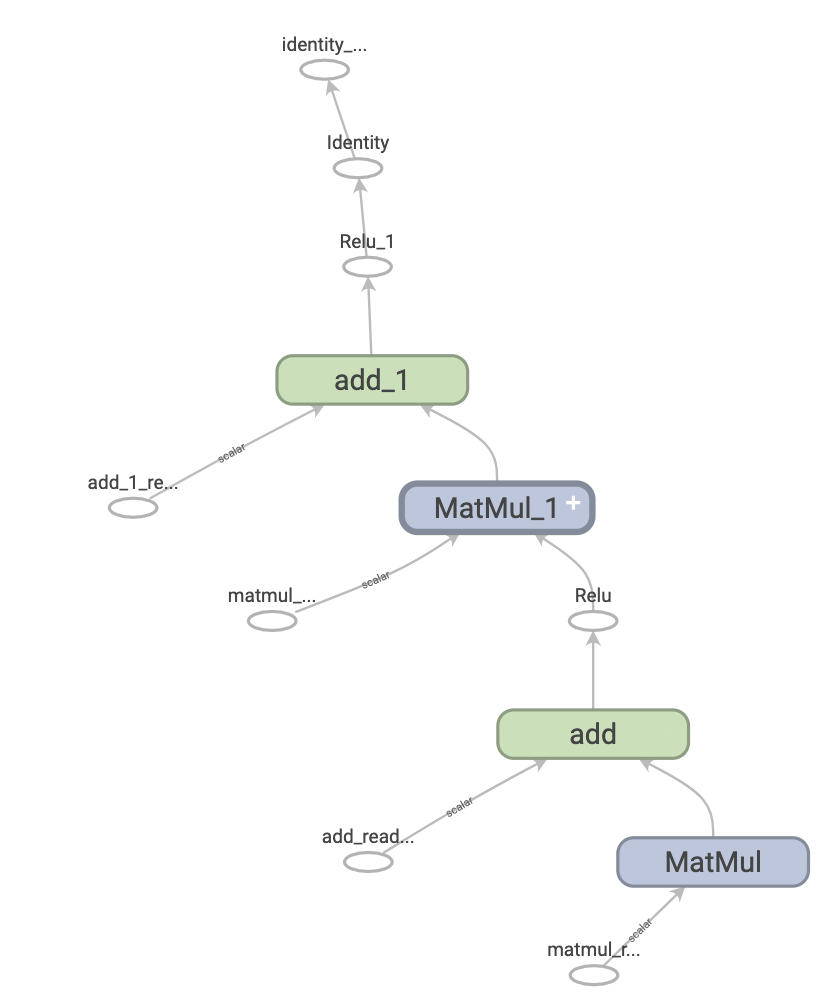
\includegraphics[width=4cm]{assets/TensorFlow_Graph_Example.png} 
                \\
                \vspace{-.1cm}
                \hspace*{-4cm}\caption{Source: tensorflow.org}
    \end{columns}
\end{frame}

\begin{frame}[fragile,allowframebreaks]{What is TensorFlow?}

        \begin{columns}[T]
        \column{0.99\textwidth}
            \vspace{1cm}
            \begin{itemize}
                \item Visualization of work by TensorBoard
                \item Natural language processing
                \item Image recognition
                \item Computational-based simulations
                \item Training and execution on GPU, CPU or TPU (Cloud)
            \end{itemize}
        
         \column{0.01\textwidth}
             \vspace{-0cm}
             \hspace*{-5cm}
             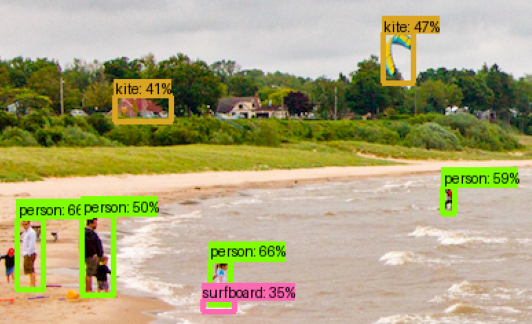
\includegraphics[width=5cm]{assets/TensorFlow_ObjectDetection(2).png}
                 \\
                 \vspace{-.1cm}
                 \hspace*{-5cm}\caption{Source: tensorflow.org}
        \end{columns}
\end{frame}

\begin{frame}[fragile,allowframebreaks]{Tensor flow: Open-source characteristics}
    \begin{itemize}
        \item Google as contributor and promoter
        \item Network of collaborators 
        \item Part of Googles business model
        \item Beyond source code: Sharing of models and datasets
        \item Customization and own ??APIs??
    \end{itemize}
\end{frame}

\begin{frame}[fragile,allowframebreaks]{Tensor flow: Google's perspective}
    \begin{itemize}
        \item Googles AI products use TensorFlow
        \item (Worldwide) collaboration
        \item Shared Datasets and ML models
        \item Googles cloud-TPUs
    \end{itemize}
\end{frame}

\begin{frame}[fragile,allowframebreaks]{Tensor flow: Pros and cons}
    \begin{itemize}
        \item Well-documented
        \item Widely used
        \item Shared Datasets and ML models
        \item Freedom to use and modify
        \item Integration in business model
        \item ???Cons???
    \end{itemize}
\end{frame}